O sistema de comunicação pode ser divido em 3 sub-sistemas principais:
\begin{itemize}
    \item Meio transmissor;
    \item Receptor;
    \item Transmissor;
\end{itemize}

No entanto, este trabalho foca exclusivamente no sistema transmissor, ilustrado pela figura \ref{fig:sistemadetrasmissao}, onde observa-se diversos elementos de que compõem o transmissor de sinal e dentre esses elementos tem-se que o amplificador de sinal é o componente de maior demanda energética, por se tratar do componente que converte a energia da fonte em energia irradiada pela antes de transmissão. Então para que o sistema de transmissão atue de maneira eficiênte é imprescindível que o trasmissor atue da maneira mais eficiênte o possivel. Conforme argumentado por \cite{Schuartz2017}.

% // TODO Refazer figura
\begin{figure}[ht!]
    \centering
    \captionsetup{justification=centering}
    \caption*{Fonte: autor}
    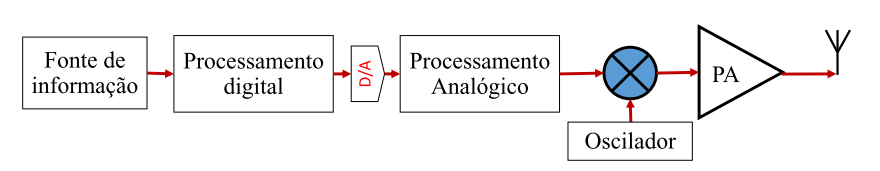
\includegraphics[width=0.5\textwidth]{sistematrasmissorpng.png}
    \caption{Sistema de transmissão simplificado}
    \label{fig:sistemadetrasmissao}
\end{figure}

Sabe-se que a evolução dos sistemas de comunicação móveis causou na implementação de diversos serviços como aplicações multimídias, desenvolvimento web, aplicações IoT. De acordo com \cite{John2016}, há uma demanda cada vez maior por sistemas de comunicação mais rápidos, robustos e eficientes, devido ao aumento no número de usuários.  Nesse contexto, melhorar a eficiência energética se mostra uma alternativa desejável tanto para aparelhos moveis, visando melhorar a autonomia da bateria, quanto para estações rádio base, uma vez que diminuiria o gasto de potência por perdas em calor. Considerando também que a largura de banda reservada para sistemas de comunicação sem fio é reduzida, torna-se desejável que ela seja utilizada da maneira mais eficiente o possível. Diante desse cenário, segundo \cite{Kenington2000}, só é possível alcançar as maiores taxas utilizando estratégias de modulações, que alterem tanto a fase quanto a amplitude de uma onda portadora em rádio frequência. Ainda segundo \cite{Kenington2000}, a modulação na amplitude, exige linearidade na transmissão afim de evitar erros e interferência na comunicação entre os usuários vizinhos. Ante esse panorama, o projetista do PARFT se depara com esse desafio, que é desenvolver um hardware eficiente, energeticamente, e com uma boa linearidade simultaneamente, uma vez que esse compromisso é conflitante, conforme descrito por \cite{Cripps2006}. Esse comportamento se deve, pois, um PARF, atua de forma eficiente, ou seja, com baixo consumo de energia, na área próxima à de saturação, que é a região em que eles operam em regimes não lineares, conforme ilustrado pela figura \ref{fig:saidaparf}.

\begin{figure}[ht!]
    \centering
    \captionsetup{justification=centering}
    \caption*{Fonte: \cite{Chavez2018}}
    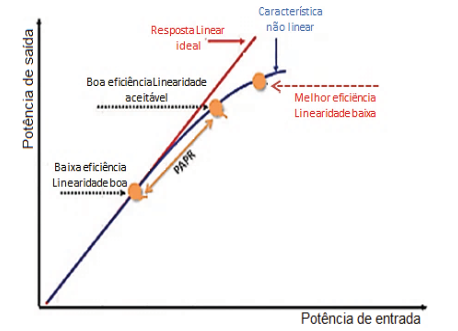
\includegraphics[width=0.5\textwidth]{curvasaidaparf.png}
    \caption{Curva de saida do amplificador}
    \label{fig:saidaparf}
\end{figure}

A fim de contornar esse obstáculo foi adicionado a cadeia de transmissão, um método de equalização de sinais, conforme argumentado por \cite{Kenington2000}. Um exemplo de técnica de linearização de sinais é a implementação de um pré-distorcedor de Sinais Digital em banda base, o qual apresenta um melhor custo-benefício \cite{Kenington2000}. Essa técnica consiste em distorcer o sinal de entrada utilizando técnicas de processamento digital, antes que esse module uma portadora, de forma compensativa à distorção causada pelo PARF. De maneira sucinta, o DPD é conectado em cascata ao PARF e é projetado de forma que apresenta a função transferência inversa ao PARF. Para isso, é necessário um modelo de alta precisão e baixa complexidade computacional, capaz de representar as características de transferência direta e inversa de um PARF. Isso significa então modelar o seu comportamento real utilizando um software.  A figura \ref{fig:cascatadpd} ilustra o processo do um pré-distorcedor digital.

\begin{figure}[h!]
    \centering
    \captionsetup{justification=centering}
    \caption*{Fonte: \cite{Chavez2018}}
    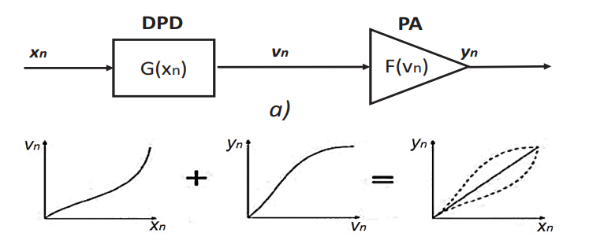
\includegraphics[width=0.5\textwidth]{DPDcascata.png}
    \caption{ilustração do pré-distorcedor em cascata}
    \label{fig:cascatadpd}
\end{figure}

Segundo \cite{John2016}, existem duas técnicas utilizadas para fazer essa modelagem. Uma consiste na descrição detalhada do PARF, que implica em uma maior complexibilidade computacional, esses modelos são conhecidos como modelos físicos. A outra abordagem é conhecida como modelo empírico, este modelo consiste em medições realizadas na entrada e na saída do PARF, e através destes dados simulam um modelo matemático do sistema. Uma das vantagens desse método é que ele não exige conhecimento prévio da estrutura do PARF e possui baixa complexidade computacional. No entanto, sua precisão pode ser ligeiramente afetada pelo modelo adotado.
% // TODO FALAR DE VOLTERRA
\section{modelagem matemáticas}



% // TODO Falar mais sobre FPGA 
\section{FPGA}
Como foi visto em \cite{Pedroni2010}, FPGAs, são uma classe de dispositivos lógicos programáveis, ou seja, permitem a reconfiguração física de seus componentes de eletrônica digital, que ocorre através de uma linguagem de descrição de hardware. 
As FPGAs consistem, basicamente, em um conjunto de sub circuitos digitais interconectados que realizam funções comuns e ao mesmo tempo, possuem alto nível de flexibilidade, portanto, pode ser utilizada para processamento de imagem em tempo real, machine learning, entre outras aplicações.
As FPGAs possuem a capacidade de sintetizar complexas arquiteturas de eletrônica digital o que acaba resultando em um funcionamento bastante paralelizado, permitindo um processamento rápido envolvendo várias portas de entrada e saída,
mas sem excluir a possibilidade de desenvolver códigos sequenciais.
A estrutura interna de uma FPGA é fundamentalmente composta por blocos lógicos interligados, dispostos como uma matriz. Cada bloco é composto por um determinado número de sub-blocos, e os sub-blocos possuem os componentes mais básicos da hierarquia. As FPGAs da Intel e da Xilinx possuem diferenças na nomenclatura dos blocos e sub-blocos, bem como na organização dos sub-blocos,
como exemplificado na Figura \ref{fig:Stratix} e na Figura \ref{fig:Ultrascale}, que mostram as FPGAS Intel Stratix X e Xilinx Ultrascale+, respectivamente. As arquiteturas fundamentalmente são semelhantes, já que a forma de matriz dos blocos e a funcionalidade dos componentes fundamentais são universais. Os blocos lógicos recebem o nome de LAB em FPGAs da Intel, e Configurable Logic Block (CLB) em FPGAs da  ilinx. Os sub-blocos são denominados ALM ou LE dependendo da FPGA da Intel, e são denominados Slices nos FPGAs da Xilinx.
\begin{figure}[h!]
    \centering
    \captionsetup{justification=centering}
    \caption*{Fonte: \cite{Pedroni2010}}
    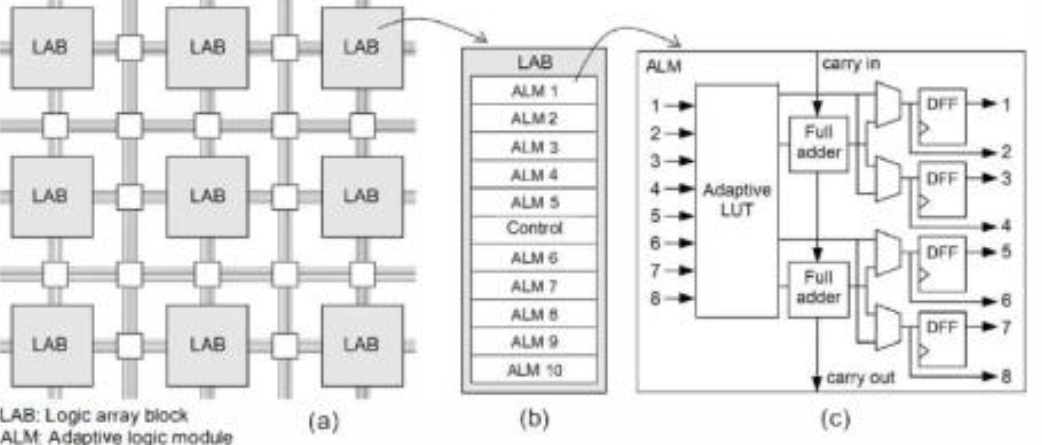
\includegraphics[width=0.5\textwidth]{FPGA Stratix X da Intel.png}
    \caption{Estrutura Interna da FPGA Stratix X da Intel}
    \label{fig:Stratix}
\end{figure}

\begin{figure}[h!]
    \centering
    \captionsetup{justification=centering}
    \caption*{Fonte: \cite{Pedroni2010}}
    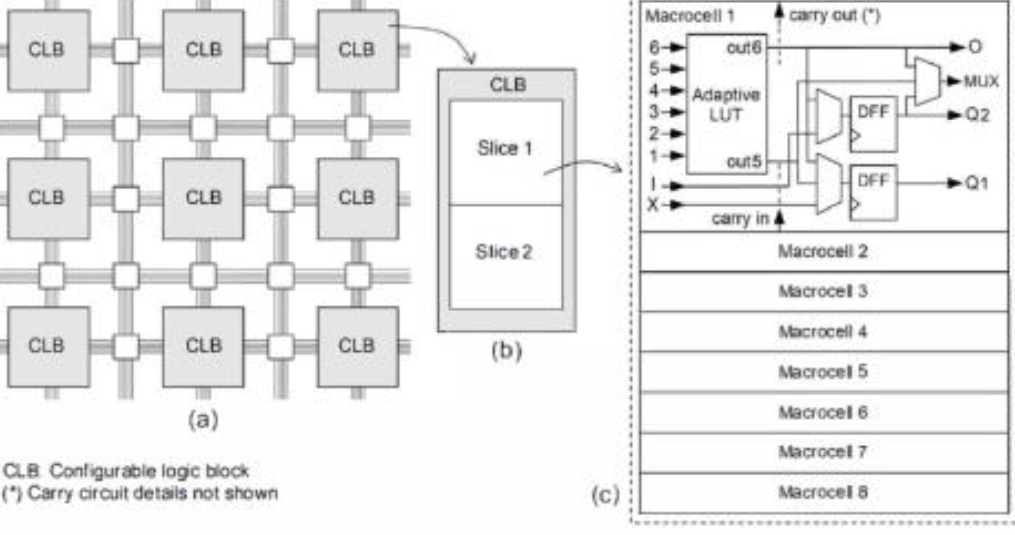
\includegraphics[width=0.5\textwidth]{FPGA Ultrascale+.png}
    \caption{Estrutura Interna da FPGA Ultrascale+}
    \label{fig:Ultrascale}
\end{figure}

Os sub-blocos das FPGAs são compostos por LUTs e registradores. As LUTs são compostas por uma árvore binária de multiplexadores 2:1, permitindo o armazenamento de uma função lógica na forma de SOP. Os registradores são os componentes síncronos dos sub-blocos. Além da estrutura mencionada, FPGAs comumente possuem diversos módulos integrados, como CPUs, DSPs, memória Flash, PLLs, que aumentam ainda mais as capacidades do FPGA.
Embora tradicionalmente algoritmos de alta segurança criptográfica tenha sido implementada como um ASIC, recentemente esta tendência vem mudando, tornando o FPGA mais popular para essas aplicações. Há várias razões para isto, o FPGA pode ser  eprogramado, levando a uma maior flexibilidade para a modificação de algoritmos e conserto de erros segundo [2]. Além de que o FPGA tem vantagens de
desempenho em tempo de design, consumo de energia, custo ou área de chip em
relação a outros sistemas baseados em microprocessadores de acordo com [3].



% // TODO Falar mais sobre FPGA 

Como mencionado anteriormente, as FPGAs são programadas utilizando uma linguagem de descrição de hardware, sendo VHDL uma das mais comuns para a síntese de circuitos integrados de alta velocidade. Foi criada por uma iniciativa financiada pelo departamento de defesa dos Estados Unidos em meados dos anos 80 e foi a primeira linguagem de descrição de hardware padronizada pela IEEE.
A estrutura de um código VHDL consiste em três partes principais: declaração de bibliotecas/pacotes, entidade e arquitetura. Na primeira parte, são listadas as bibliotecas e pacotes necessários para o projeto. As bibliotecas padrão incluem a std e a work. A entidade, que é a interface do sistema, descreve as entradas e saídas e é dividida em duas partes: parâmetros e conexões. Os parâmetros são valores constantes, como a largura de um barramento, que são declarados como genéricos. As conexões, por sua vez, definem a transferência de informações e correspondem aos pinos de entrada e saída do circuito. Já a arquitetura é a parte principal do sistema, onde o circuito é descrito. Nessa seção, são definidas as atribuições, operações lógicas e aritméticas, comparações, entre outros. Há também uma parte declarativa da sintaxe, que apresenta uma ampla variedade de declarações possíveis.
Sendo assim, circuitos digitais para processamento de sinais em tempo real são muito utilizados em sistemas de comunicações sem fio. Um exemplo de aplicação são os pré-distorcedores para transmissores sem fio. Os PDs são baseados em operações matemáticas que envolvem uma grande quantidade de operações de soma, produto e tabelas de busca. Devido às rigorosas exigências de frequência de operação, torna-se fundamental a paralelização das operações necessárias. Nesse contexto, as FPGAs são uma alternativa viável para a implementação de circuitos pré-distorcedores.